\documentclass{beamer}

\usepackage[overlay,absolute]{textpos}

\usetheme{Copenhagen}
\usecolortheme{rose}

\title[Bioinformatics Workshop]{Getting Started in the Flaherty Lab}
\author[T. Zhang]{Tete Zhang}
\institute[WPI]{
    Department of Bioinformatics and Computational Biology\\
    Worcester Polytechnic Institute\\
    Worcester, MA 01609\\[1ex]
    \texttt{tzhang3@wpi.edu}
}
\date[May 2014]{May 29, 2014}

\begin{document}

%--- title page ---
\begin{frame}[plain]
    \titlepage
\end{frame}

%---data management title page---
\begin{frame}{Getting Started in the Flaherty Lab}
\LARGE\textbf{Data Management}
	\begin{itemize}
  \item\LARGE Bench Data
  \item\LARGE Fridge Data
  \item\LARGE Freezer Data
	\end{itemize}
\end{frame}

%---data management big picture---
\begin{frame}{Data Management}
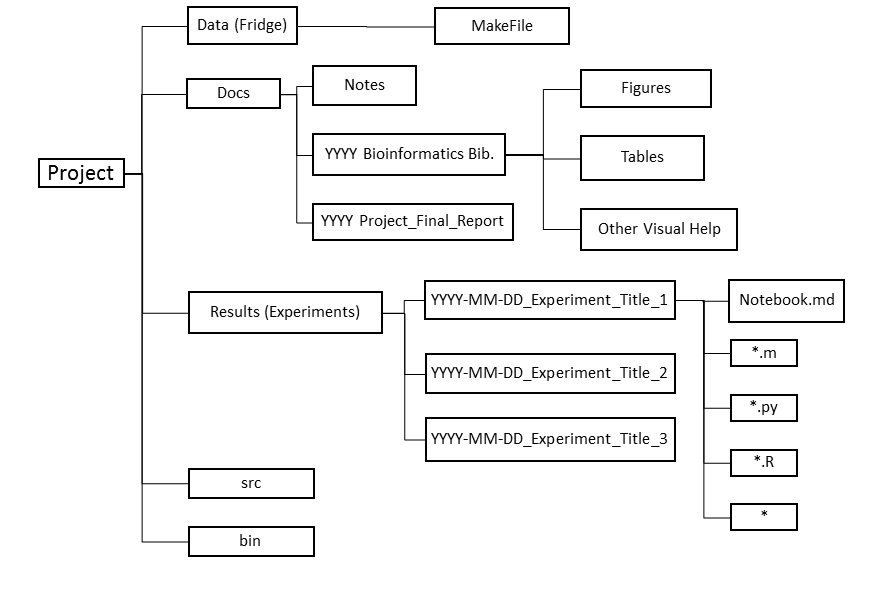
\includegraphics[width=4in, height=3in]{structure.png}
\end{frame}

%--- data fridge---
\begin{frame}{Data Management - Data Fridge}

\begin{columns}[t] % contents are top vertically aligned
     \begin{column}[T]{4cm}
     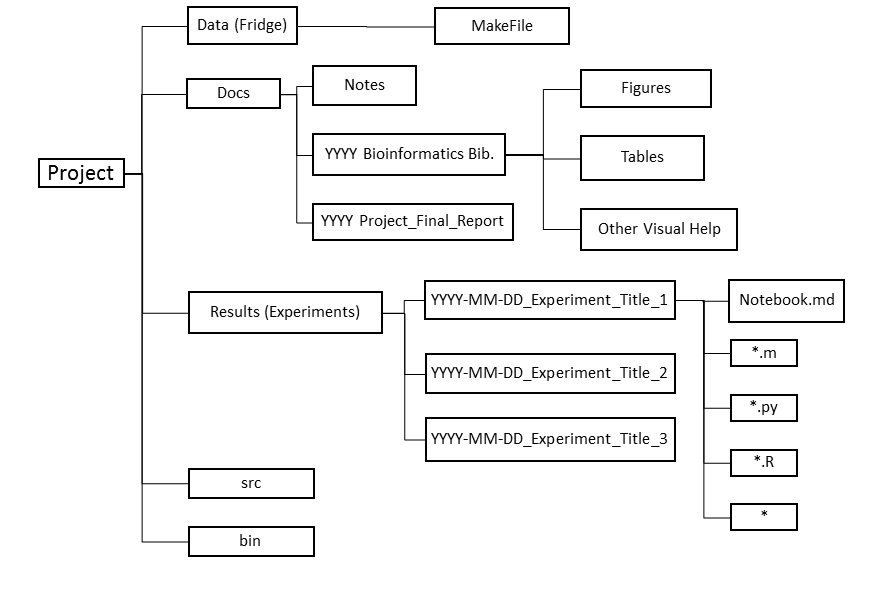
\includegraphics[width=2in, height=2.5in]{structure.png}
     \end{column}
     \begin{column}{6cm}
     
    	\begin{textblock}{8}(7.3,3)
    		\visible<1->{
      		\textbf{Data Fridge}
      		
      		\begin{itemize}
		\item{Makefile}
		\item{target:dependent
		
			[tab] rules}
		\item{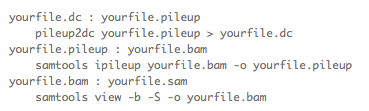
\includegraphics[width=2.5in, height=1in]{makefile.png}}
		\end{itemize}
		
                  }
	\end{textblock}
              
     \end{column}
     \end{columns}
     
\end{frame}

%--- docs ---
\begin{frame}{Data Management - Docs}
	\begin{itemize}
\item\LARGE{Notebook}
\item{Figures and Tables}
\item{Project Final Report}
	\end{itemize}
\end{frame}

%--- source ---
\begin{frame}{Data Management - src (source)}
	\LARGE{Completed code for your data analysis program.}
\end{frame}

%--- bin ---
\begin{frame}{DataManagement - bin}
	\LARGE{Executable files, such as:}
		\begin{itemize}
	\item\LARGE{Resources helpful to the experiment}
	\item{Compiled programs - execute with one command}
		\end{itemize}
\end{frame}

%--- GIT title page---
\begin{frame}{Getting Started in the Flaherty Lab}
\LARGE\textbf{Version Control}
	\begin{itemize}
  \item\LARGE Why Version Control?
  \item\LARGE What are the options for Version Control?
  \item\LARGE Why GIT?
	\end{itemize}
\end{frame}

%--- GIT ----
\begin{frame}{Version Control - GIT}
	\begin{itemize}
  \item\LARGE{GIT GUI or Command Line}
  \item\LARGE{clone, fetch, pull}
  \item\LARGE{stage, commit, push}
  \item\LARGE{Conflict Management}
	\end{itemize}
\end{frame}

%--- Flaherty Lab Environment title page ---
\begin{frame}{Getting Started in the Flaherty Lab}
\LARGE\textbf{Flaherty Lab Environment}
\end{frame}

%--- Flaherty Lab background ---
\begin{frame}{Flaherty Lab Environment}
          \begin{itemize}
  \item\LARGE Redwood Server
  \item\LARGE Amazon Machine Image
  \item\LARGE Starcluster? MPI? What else?
	\end{itemize}
\end{frame}

%--- Redwood Server ---
\begin{frame}{Flaherty Lab Environment - Redwood Server}
	\begin{itemize}
  \item\LARGE{Flaherty Lab Linux Server for Computation}
  \item\LARGE{64 core + 256GB RAM}
  \item\LARGE{9TB high speed drive + 1TB solid state drive via NFS}
	\end{itemize}
\end{frame}

%--- AMI ---
\begin{frame}{Flaherty Lab Environment - Amazon Machine Image (AMI)}
          \begin{itemize}
  \item\LARGE{When you need more than 64 cores for calculation..}
  \item\LARGE{numpy, scipy, h5py, pytables, matplotlib, pyramid, scikit-learn, pandas, statsmodels, networkx, theano, gdal, pysal, and shapely}
  \item\LARGE{on-demand price: 0.145 dollar per worker per hour
  
  spot instance price: 0.018 dollar per worker per hour}
	 \end{itemize}
\end{frame}

%--- end page---
\begin{frame}{Getting Started in the Flaherty Lab}
\LARGE\textbf{Thank you!}
\end{frame}

\end{document}